\chapter{Implementation}
Für die Implementation dieser Bachelorarbeit wurden die in vorherigem Kapitel \ref{ch:konzepte_architektur} beschrieben Konzepte angewendet.
\section{XML Daten Import}
Um mit den grossen Datenmengen in den vorhandenen XML Dateien effizient zu arbeiten, müssen diese Daten in eine Datenbank importiert werden. Dafür wurde ein Import Formular im Web Interface integriert, das im Hintergrund die Daten an einen Web Service sendet, der für den Import zuständig ist. Die Daten werden direkt beim Import aufbereitet, so dass die Abfrage der Daten schneller ist.
\section{Tiling der Daten}
\label{sec:tilingdataimplementation}
Während des Imports werden zwei verschiedene Vorberechnungen durchgeführt. Mit Hilfe dieser vorbereiteten Informationen ist es möglich, effizienter die Daten zu filtern. Dadurch wird die Antwortzeit einer Anfrage deutlich verkürzt.
\subsection{QuadKey}
Die erste Vorbereitung ist die Berechnung des QuadKeys. Wie in Kapitel \ref{ch:datentiles} \nameref{ch:datentiles} beschrieben, können mit Hilfe des QuadKey einzelne Bereiche der Welt eindeutig identifiziert werden. Wenn nun eine Anfrage an den Server gesendet wird, in der die Daten eines spezifischen QuadTiles angefordert werden, müssen die Links ebenfalls einen QuadKey besitzen um danach zu filtern. Dafür werden die QuadKeys der beiden Nodes berechnet, die zu einem Link gehören. Der gemeinsame Prefix stellt nun den kleinst möglichen QuadKey dar, in den der gesamte Link hineinpasst.\\
Wie in Abbildung \ref{pic:example_quadtile} bei Link 2 ersichtlich, kann sich eine Strasse auch in einem QuadTile befinden, ohne dass sich beide Nodes in diesem Quadtile befinden. In diesem Beispiel hat Link 1 einen QuadKey von 010 und Link 2 von 01. Damit nun der Link 2 bei einer Abfrage der Daten des QuadTiles 010 auch mitgeliefert wird, müssen alle Strassen, die eine QuadKey besitzen, der einen Prefix des angeforderten QuadKeys darstellt, auch mitgeliefert werden. D.h. dass nun für die Abfrage des QuadTiles 010 alle Strassen, die den QuadKey 010, 01, 0 oder sogar einen leeren QuadKey \glqq{}\grqq{} besitzen mitgeliefert werden.
\begin{figure}[H]
\centering
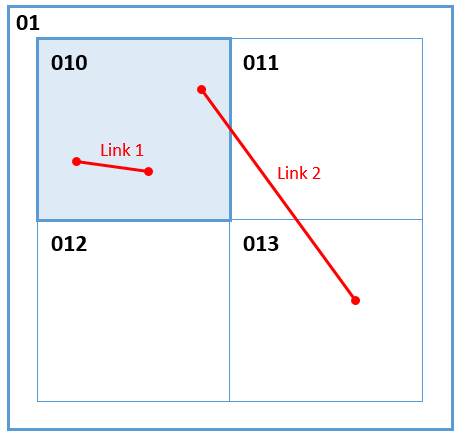
\includegraphics[height=9cm]{images/QuadTile_example.PNG}
\caption{Beispiel QuadTile}
QuadKey Link 1: 010\\QuadKey Link 2: 01
\label{pic:example_quadtile}
\end{figure}
\noindent
Der QuadKey ist eine sehr gute Technik, um die Daten auf der Karte zu adressieren und dadurch eine Filterung der Daten durchzuführen. Zudem hat diese Technik den Vorteil, dass sichergestellt ist, das alle Links, die auf einem gewissen QuadTile ersichtlich sind, sicher mitgeliefert werden.\\
Ein Nachteil dieser Technik ist es, dass bei höheren Zoomlevels Daten mitgeliefert werden, die bei einem vorherigen QuadTile bereits mitgeliefert wurden. Das User Interface verhindert zwar das neu Zeichnen von Duplikaten, jedoch werden dadurch viele Daten übertragen, die bereits gezeichnet sind und dadurch überflüssig sind.
\newpage
\subsection{MinLevel}
Zusätzlich zu dem QuadKey wird beim Import noch für jeden Link der Mindest-Level (MinLevel) berechnet. Denn nur mit dem QuadKey würden alle Strassen in der aktuell angezeigten Bounding Box geladen werden, auch die eher kleineren Nebenstrassen. Aus diesem Grund wird beim Import ein MinLevel berechnet, der besagt, ab welchem Zoom Level in der Karte diese Strasse geladen wird. Dadurch ist es möglich eine Strasse nach ihrer Wichtigkeit zu gewichten und erst ab einem bestimmten Zoomlevel anzuzeigen. \\
Bei der Berechnung dieses Mindest-Levels wird in erster Linie auf die maximale  Geschwindigkeit geachtet. Die Geschwindigkeit sagt sehr viel über die Wichtigkeit der Strasse selbst aus. Eine Strasse mit einer hohen maximalen Geschwindigkeit, wie z.B. eine Autobahn, wird in diesem System als wichtig erachtet und dadurch bereits auf einem niedrigeren Zoomlevel angezeigt. Beim Level 10 und 14 wurden noch weitere Kriterien verwendet um eine feinere Skalierung zu erhalten.\\
Der MinLevel einer Strasse wird wie folgt berechnet:\\[0.3cm]
\begin{tabular}{l c l} 
Level 10 & => & Geschwindigkeit > 30 m/s und Anzahl Spuren > 2 \\ 
Level 11 & => & Geschwindigkeit > 30 m/s  \\ 
Level 12 & => & Geschwindigkeit > 23 m/s \\ 
Level 13 & => & Geschwindigkeit > 14 m/s \\ 
Level 14 & => & Geschwindigkeit > 13 m/s und Kapazität >= 4000  \\ 
Level 15 & => & Geschwindigkeit > 13 m/s \\ 
Level 16 & => & Der Rest \\ 
\end{tabular} 
\section{Performance Optimierungen}
Die Performance ist ein sehr wichtiger Faktor in dieser Arbeit. Ohne starke Performance kann die grosse Datenmenge in diesem Projekt nicht effizient dargestellt werden. Aufgrund dessen, wurde einiges an Zeit in die Optimierung investiert. Zwei wichtige Faktoren haben grossen Einfluss auf die Performance dieser Web Applikation. Zum einen ist dies die Antwortzeit der einzelnen Abfragen der Daten. Diese Antwortzeit konnte durch mehrere Optimierungen, die in diesem Kapitel genauer beschrieben werden, deutlich verbessert werden. Dadurch konnten die nicht-funktionalen Anforderungen aus dem Kapitel \ref{ch:NFRs} eingehalten werden.\\
Ein weiterer grosser Faktor ist das Rendering der Daten im Browser. In höheren Zoomlevels werden bis zu mehreren Tausend Links und Nodes im Browser dargestellt. Der Browser benötigt für das Rendering doch eine gewisse Zeit, auf die der Entwickler keinen grossen Einfluss hat. Es kann lediglich darauf geachtet werden, dass keine redundante Informationen vom Browser gerendert werden müssen.
\subsection{Caching}
Für die Anzeige der Strassen und Nodes werden sehr viele Daten übertragen. Damit die Daten bei mehrmaligem Anfragen nicht jedes Mal übertragen werden müssen, wird Clientseitiges Caching eingesetzt.\\
Der Server gibt dem Client vor, wie er die Daten zwischenspeichern soll. Dafür wird bei jeder Antwort eine maximales Alter der Daten gesetzt. Wie in Abbildung \ref{pic:browser_cache} ersichtlich, speichert der Client die Daten in seinen lokalen Zwischenspeicher (Cache) und verwendet diese, solange das maximale Alter von einer Stunde noch nicht erreicht ist. Dies macht Sinn, weil sich die Stammdaten des Verkehrsmodells nur sehr selten ändern. Erst nach Auflauf dieser Stunde sendet der Browser erneut eine Anfrage an der Server.
\begin{figure}[H]
\centering
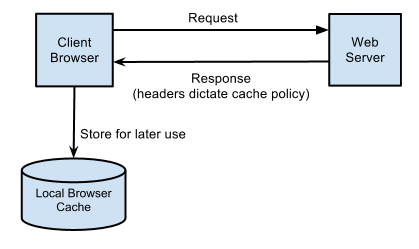
\includegraphics[height=6cm]{images/browser_cache.jpg}
\caption{Browser Zwischenspeicher Request (Cache) \cite{HTTPCacheHeaders}}
\label{pic:browser_cache}
\end{figure}
\noindent
Nun liegt es am Server zu prüfen, ob die Daten, die sich im Cache des Clients befinden, noch aktuell sind. Dafür wird mit einem HTTP Entity Tag gearbeitet \cite{WikipediaETag}. Dieser setzt sich aus der x- und y-Koordinate, dem Zoom Level sowie aus dem Zeitstempel der letzten Bearbeitung der Daten zusammen. Durch diese unterschiedlichen Informationen ist der Entity Tag für jeden QuadTile eindeutig. Durch das zusätzlich Verwenden des Zeitstempels ist auch sichergestellt, dass sich der Entity Tag unterscheidet, sobald eine Änderung in den angeforderten Stammdaten auf dem Server vorliegt.\\
Jede Antwort, die zuvor an den Client gesendet wurde, wird mit diesem HTTP Entity Tag versehen. Beim erneuten Anfragen der Daten, wird dieser Entity Tag vom Client mitgesendet und mit dem berechneten, aktuellen Entity Tag der Daten auf dem Server verglichen. Wie in Abbildung \ref{pic:browser_etag} ersichtlich, wird vom Server der HTTP Status 304 (Not Modified) \cite{W3HttpStatus} gesendet, falls diese identisch sind. Dadurch weiss der Client, dass seine Daten noch aktuell sind. Wurden die Stammdaten auf dem Server geändert, stimmen die Entity Tags aufgrund des Zeitstempels der letzten Bearbeitung nicht mehr überein und der Server sendet die neuen Daten an den Client. Diese Daten werden dann vom Client wieder für eine Stunde zwischengespeichert und anschliessend beginnt das Ganze von vorne.
\begin{figure}[H]
\centering
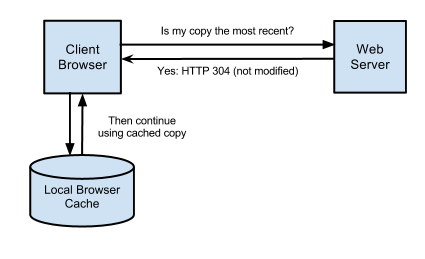
\includegraphics[height=6cm]{images/browser_etag.jpg}
\caption{HTTP Entity Tag Request \cite{HTTPCacheHeaders}}
\label{pic:browser_etag}
\end{figure}
\noindent
Durch dieses Verfahren ist sichergestellt, dass das Übertragen von Daten möglichst reduziert wird und dadurch viel Performance gewonnen wird. Diese gewonnene Performance wird erst beim längeren Verwenden der Applikation ersichtlich, sobald bereits geladene Daten nicht mehr erneut geladen werden müssen.
\subsection{Erneutes Zeichnen}
Die verwendete Library \glqq{}Leaflet GeoJSON Tile Layer\grqq{} \cite{LeafletGeoJSON}, die für das Abfragen der Daten in Tiles verantwortlich ist, ist standardmässig so entwickelt, dass die Daten auf jedem Zoom Level neu gezeichnet werden. Im Rahmen dieser Arbeit wurde die Funktionalität erweitert, sodass die Strassen beim hineinzoomen bestehen bleiben und lediglich die neuen Strasse dazu gezeichnet werden. Ebenfalls wurde die Library so angepasst, dass  beim herauszoomen alle Strassen, die auf einem höheren Zoomlevel gezeichnet wurden, wieder entfernt werden. Dafür werden alle Schlüssel der gezeichneten Strassen mit dem dazugehörigen Zoomlevel, auf dem sie gezeichnet wurden, in eine Map< Zoomlevel, List<Schlüssel> > abgelegt. Dadurch kann die Library beim herauszoomen alle Schlüssel, die zu einem Zoomlevel gehören, löschen.
\subsection{Datenbank Index \& Redundanz}
TODO
\section{Handler}
evtl. TODO
\subsection{UndoRedoHandler}
evtl. TODO
\subsection{ChangesetHandler}
evtl. TODO
\subsection{ChangesetStorageHandler}
evtl. TODO
\section{UI - Implementation}
\section{Testing}
\section{Infrastruktur}
TODO
\subsection{Docker}
TODO
\subsection{Load Balancing}
TODO